\section{Seno e Cosseno da Soma}
\begin{frame}
\frametitle{Fórmulas de Adição de Arcos} 

\begin{proposicao}
Sejam $\alpha, \beta \in \R$. Então
$$\cos \paren{\alpha + \beta} = \cos \alpha \cdot \cos \beta - \sen
\alpha \cdot \sen \beta$$ e
$$\sen \paren{\alpha + \beta} = \sen \alpha \cdot \cos \beta +\sen \beta \cdot
\cos \alpha.$$
\end{proposicao}\pause
Da paridade das funções seno e cosseno seguem que:
$$\cos \paren{\alpha - \beta} = \cos \alpha \cdot \cos \beta + \sen
\alpha \cdot \sen \beta$$ e
$$\sen \paren{\alpha - \beta} = \sen \alpha \cdot \cos \beta - \sen \beta \cdot
\cos \alpha.$$

Além disso, temos os casos particulares
$$\cos \paren{2\alpha } = \cos^2 \alpha  - \sen^2 \alpha \ \ \text{ e }
\ \ \sen \paren{2\alpha } = 2\sen \alpha \cdot \cos \alpha.$$ As
fórmulas acima valem para todo $\alpha, \beta \in \R$.


\end{frame}

%------------------------------------------------------------------------------------------------------------
\begin{frame}
\frametitle{Rotação de Pontos no Plano Cartesiano} 

Considere o ponto $A = (x, y) \in \R^2$ e chame de $\alpha$ o ângulo
formado pelo segmento $OA$ com o eixo positivo de $x$. A função
$T_{\theta} : \R^2 \to \R^2$  tal que
$$T_{\theta}\paren{x, y} = \paren{x\cdot \cos \theta - y\cdot \sen \theta, x\cdot \sen \theta + y\cdot \cos
\theta}$$ é a rotação de ângulo $\theta$ do ponto $A = (x,y)$ em
torno da origem.

\begin{center}
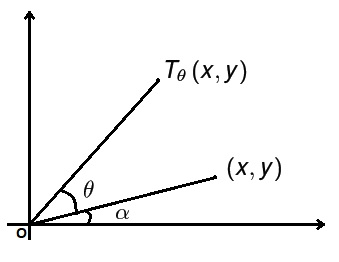
\includegraphics[width=5.5cm]{figures/rotacao.jpg}
\end{center}


\end{frame}

%------------------------------------------------------------------------------------------------------------